% Native editable composition from one verified, unchanged IDE capture.
\begin{figure}[htbp]
\centering
\sbox0{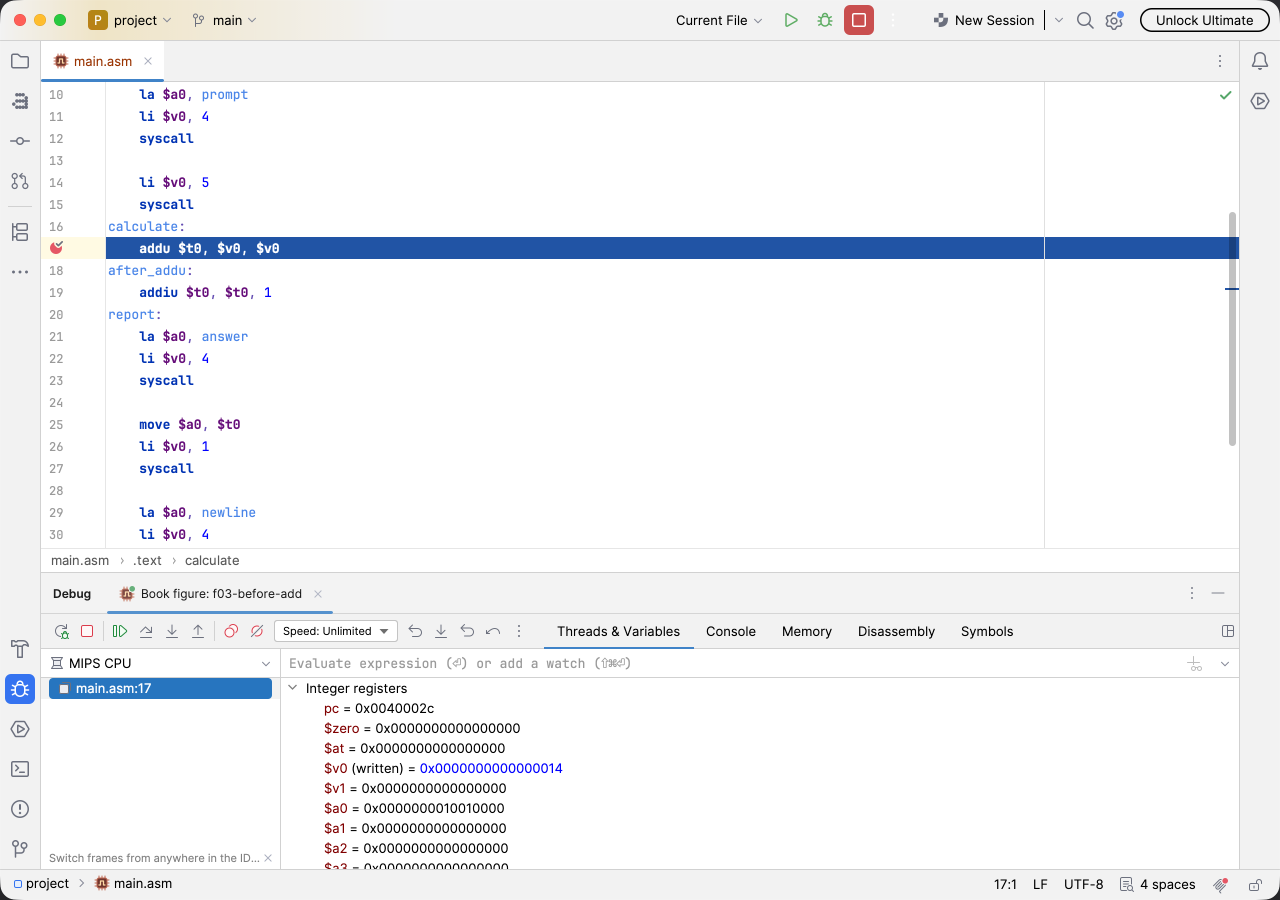
\includegraphics[artifact]{packages/001-console-calculation/captures/f03-before-add/raw.png}}
\edef\MARSconsolebeforeaddsourceLeft{\the\dimexpr0.036718750\wd0\relax}
\edef\MARSconsolebeforeaddsourceBottom{\the\dimexpr0.707777778\ht0\relax}
\edef\MARSconsolebeforeaddsourceRight{\the\dimexpr0.611718750\wd0\relax}
\edef\MARSconsolebeforeaddsourceTop{\the\dimexpr0.236666667\ht0\relax}
\edef\MARSconsolebeforeaddvalueLeft{\the\dimexpr0.246093750\wd0\relax}
\edef\MARSconsolebeforeaddvalueBottom{\the\dimexpr0.132222222\ht0\relax}
\edef\MARSconsolebeforeaddvalueRight{\the\dimexpr0.553906250\wd0\relax}
\edef\MARSconsolebeforeaddvalueTop{\the\dimexpr0.838888889\ht0\relax}
\begin{tikzpicture}[alt={Two annotated Debug details before addu t0 v0 v0. The current blue source line is addu. The visible v0 register is hexadecimal 0000000000000014, decimal 20, returned by the integer-input service. The value 20 has not yet been doubled.}]
\node[anchor=north west,inner sep=0,font=\small\bfseries] (source-title) at (6mm,0) {The next instruction reads the input twice};
\node[anchor=north west,inner sep=0] (source) at ([yshift=-1mm]source-title.south west) {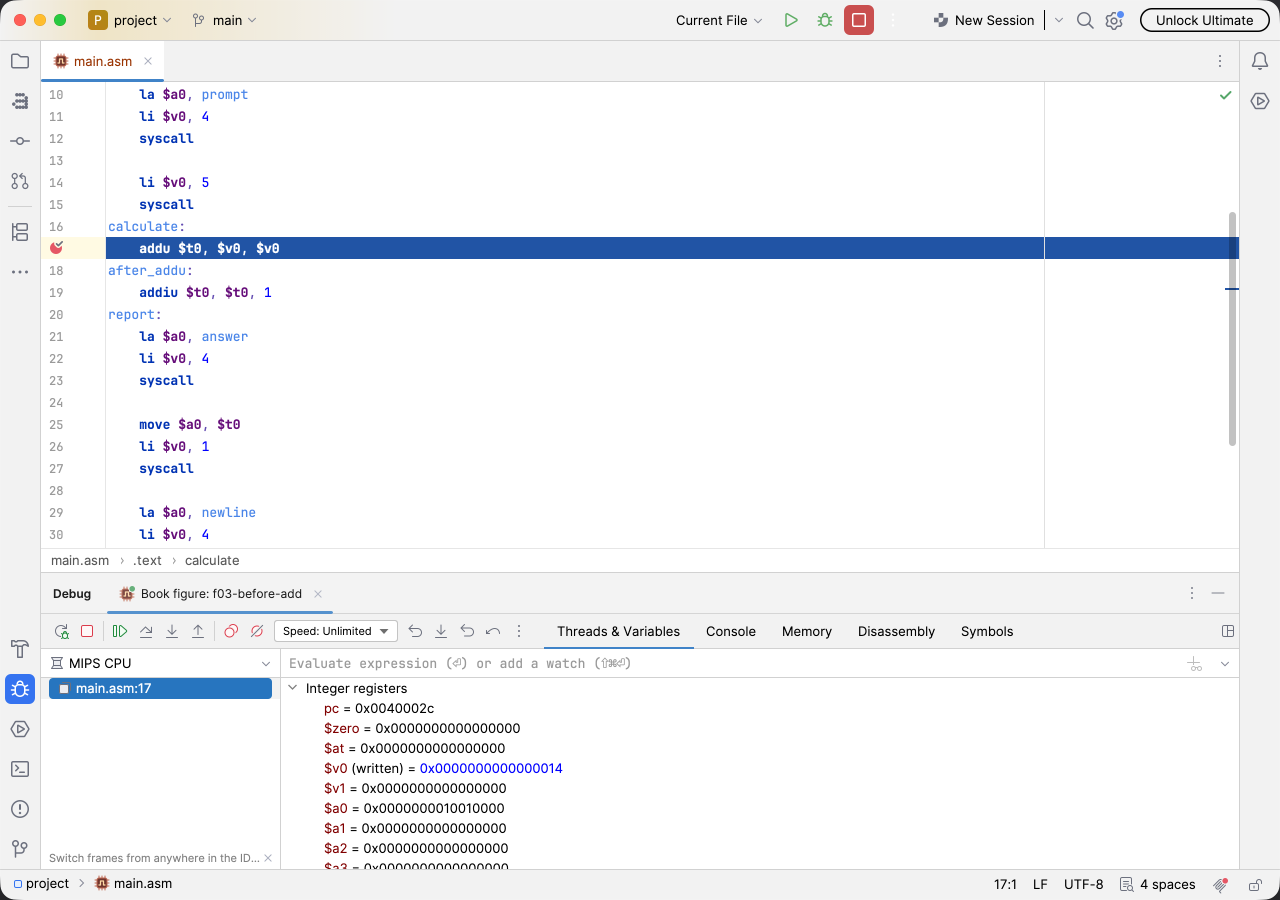
\includegraphics[width=0.7\linewidth,artifact,trim={\MARSconsolebeforeaddsourceLeft{} \MARSconsolebeforeaddsourceBottom{} \MARSconsolebeforeaddsourceRight{} \MARSconsolebeforeaddsourceTop{}},clip]{packages/001-console-calculation/captures/f03-before-add/raw.png}};
\begin{scope}[shift={(source.south west)},x={($(source.south east)-(source.south west)$)},y={($(source.north west)-(source.south west)$)}]
\draw[black,line width=0.7pt] (0.135555556,0.080000000) rectangle (0.515555556,0.520000000);
\node[draw=black,fill=white,circle,inner sep=1.5pt,font=\footnotesize] at ($(0.135555556,0.520000000)+(-3mm,0)$) {1};
\end{scope}
\node[anchor=north west,inner sep=0,font=\small\bfseries] (value-title) at ([yshift=-2mm]source.south west) {The input service returned decimal 20};
\node[anchor=north west,inner sep=0] (value) at ([yshift=-1mm]value-title.south west) {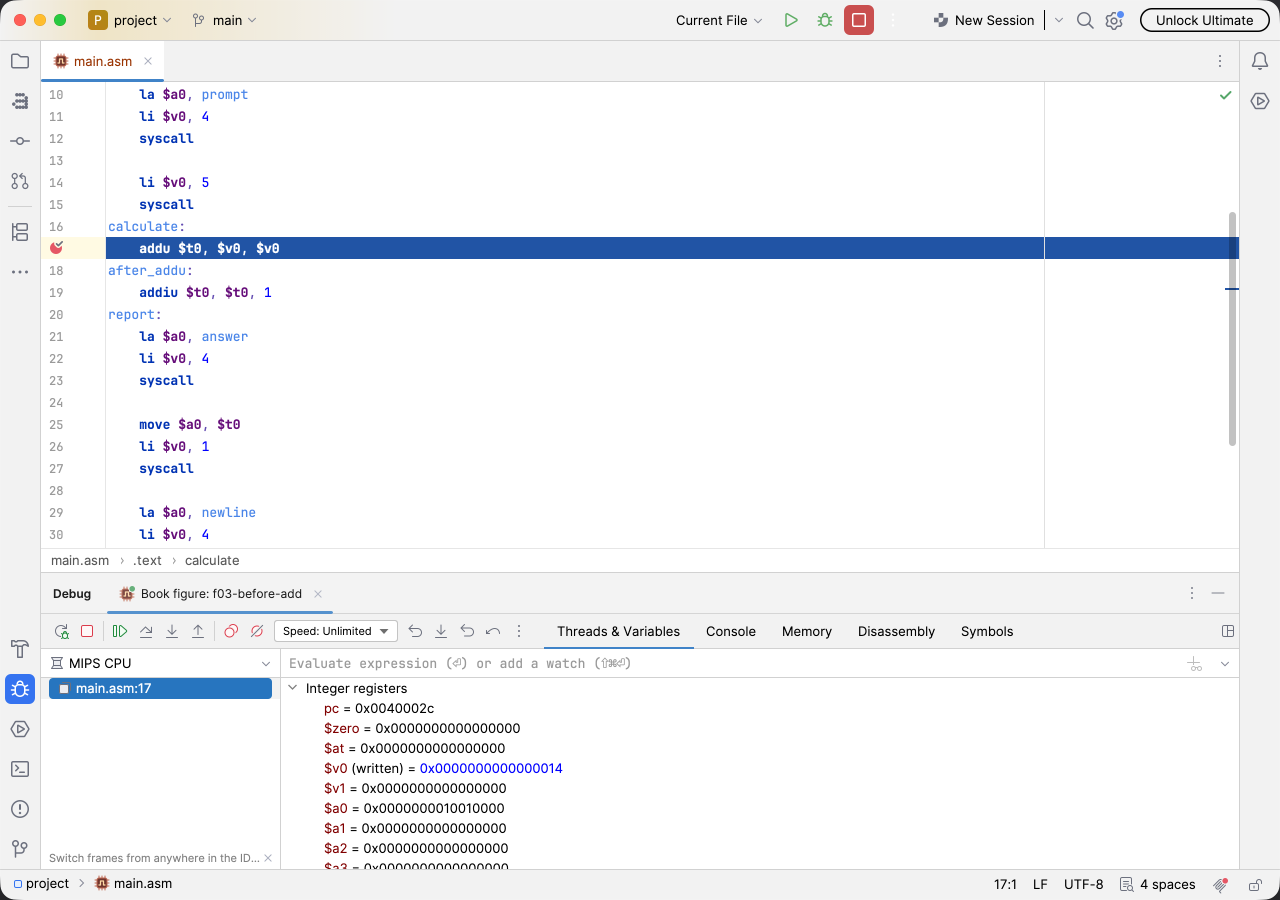
\includegraphics[width=0.53\linewidth,artifact,trim={\MARSconsolebeforeaddvalueLeft{} \MARSconsolebeforeaddvalueBottom{} \MARSconsolebeforeaddvalueRight{} \MARSconsolebeforeaddvalueTop{}},clip]{packages/001-console-calculation/captures/f03-before-add/raw.png}};
\begin{scope}[shift={(value.south west)},x={($(value.south east)-(value.south west)$)},y={($(value.north west)-(value.south west)$)}]
\draw[black,line width=0.7pt] (0.023437500,0.115384615) rectangle (0.976562500,0.884615385);
\node[draw=black,fill=white,circle,inner sep=1.5pt,font=\footnotesize] at ($(0.023437500,0.884615385)+(-3mm,0)$) {2};
\end{scope}
\end{tikzpicture}
\par\smallskip
\begin{minipage}{\linewidth}
\small
\begin{enumerate}
\item The blue line identifies the next instruction. \texttt{addu \$t0, \$v0, \$v0} reads \texttt{\$v0} twice and writes their sum to \texttt{\$t0}. At this stop it has not performed that write.
\item The register view uses hexadecimal. \texttt{0x14} is decimal 20. Service five has already returned this input in \texttt{\$v0}; the register no longer contains the service selector five.
\end{enumerate}
\end{minipage}
\caption{Before the doubling instruction. The highlighted instruction has not executed yet.}
\label{capture:001-console-calculation-f03-before-add}
\end{figure}
